% !TeX spellcheck = en_GB
\chapter{Methods}

This section discusses the optical setup, describes a number of ways in which one can perform polarisation microscopy and introduces pSTED, a method to increase the microscope resolution in the polarisation domain. Finally, the samples used in this thesis will be discussed.

\section{Microscope setup}

\begin{figure}[h!]
	\centering
	\includegraphics[width=\linewidth]{microscope layout.pdf}
	\caption{
		Schematic overview of the Tegenfeldt microscope. The sample is located in a microscope housing on the bottom right (outside this figure). FC1 and FC2 are swappable filter cubes. Half-wave and quarter-wave plates are denoted $ \lambda/2 $ and $ \lambda/4 $, respectively. Dashed lines represent the light path, except those that go to the TCSPC (those are digital connections). Red components are specifically designed to alter light polarisation. The components marked in blue (in the pSTED module) were installed during the project.
	}
	\label{fig:layout}
\end{figure}

\begin{figure}
	\centering
	\includegraphics[width=.75\linewidth]{microscope-photo-annotated.png}
	\caption{
		Photo of the optical enclosure, in the same orientation as \autoref{fig:layout}. The pSTED module is not shown. Waveplates are highlighted in red, and the beam paths of the 640 laser, the 775 nm laser, and the emission light are highlighted in blue, red, and green, respectively.
	}
	\label{fig:microscope photo}
\end{figure}

In short, the Tegenfeldt STED microscope is a scanning confocal fluorescence microscope constructed by Abberior Instruments GmbH (Germany). It features two excitation lasers (at 561~nm and 640~nm) and one depletion laser at 775~nm for two-channel confocal or STED microscopy. It also contains a time-correlated single photon counter (TCSPC) for fluorescence lifetime imaging microscopy (FLIM) and a highly sensitive photomultiplier tube (PMT). Refer to Figures \ref{fig:layout} and \ref{fig:microscope photo} for the layout of these optical elements. Samples are located inside an inverted Nikon microscope body (Ti-E, not shown in the figure) equipped with a piezo stage (M-687 PILine XY-stage system and P-736 PInano (Physik Instrumente) Z Microscope Scanner), a 60x, 1.4~NA oil immersion objective (Nikon Plan Apo) and a QUADScan beam scanner (Cambridge Technology).

The microscope has a number of waveplates that are responsible for manipulating the polarisation of laser light and fluorescence light (highlighted in red in \autoref{fig:layout}). In normal operation, all lasers are circularly polarised at the sample plane, but the waveplates in the excitation modules (640 and 561~nm) can be controlled through software to excite the sample with linearly polarised light. The waveplates in the STED module cannot, and therefore the depletion beam is always circularly polarised. Part of this project involved working with a linearly polarised depletion beam, so two waveplates were added in the STED module to achieve that result. Finally, a polarising beam splitter can be inserted into one of the filter cube housings in front of the APDs to measure the polarisation of photons emitted by fluorescence in the sample. In order for this measurement to make any sense, the waveplates in the detection module had to be set up correctly. More information about the laser and detection modules can be found in \autoref{chap:characterisation}.

\section{Conventional polarisation microscopy: acquisition and analysis}
\label{sec:pol analysis}
 
Because the current setup offers so much control over the light polarisation on both the excitation and detection ends, one can perform polarisation microscopy in several different ways:
\begin{enumerate}
	\item Measuring the intensity of emission components parallel and orthogonal to linearly polarised excitation ($ I_\parallel $ and $ I_\perp $). This is a very established method of polarisation microscopy, and allows for making anisotropy images, where every pixel is calculated according to
	\begin{equation}
		r=\frac{I_\parallel - I_\perp}{I_\parallel + 2I_\perp}.
	\end{equation}
	
	One advantage of this method is that it requires only one acquisition, whereas the following require multiple.
	
	\item Detection of emission polarised at different angles after circularly polarised (or non-polarised) excitation.
	
	\item Detection of total emission intensity as a function of the polarisation angle of excitation light.
\end{enumerate}

Methods 1 and 2 require the POL cube to be placed in one of the filter cube housings. When placed in FC1, the POL cube reflects $ s $-polarised light (vertical) into APD1 and transmits $ p $-polarised light (horizontal) to be collected by APD2. Unfortunately, we cannot use these methods yet, since they rely on the action of the detection waveplates, even if they are not actively used during the acquisition. Once we do, however, the waveplates can be used to sample more than two angles during an acquisition. This is necessary to distinguish between light polarised along \ang{+-45}, since these two angles give exactly the same intensity when sampling at \ang{0} and \ang{90} degrees.

The last method is not subject to those constraints, and is already achievable on the Tegenfeldt microscope. I have carried out some measurements and wrote code to analyse that data. The process of acquiring and analysing these images goes as follows:
\begin{enumerate}
	\item Acquire a stack of images at different excitation polarisation angles $ \theta_n $, resulting in a three-dimensional array of intensity values $ I_{nxy} $.
	\item Align images in this stack with each other, as the excitation beam seems to move as a function of polarisation angle.
	\item Compensate for photobleaching.
	\item For every pixel, calculate the Fourier coefficient corresponding to a \ang{180}-periodic signal.
	\item Based on that information, construct a new image in the HSV (hue, saturation, value) colour space where pixel colour depends on the polarisation direction, the saturation shows the degree of polarisation and the brightness (value) shows the total intensity of a pixel. 

\end{enumerate}

For more information, refer to \autoref{sec:polarisation microsocpy protocol}. The results of this method are presented in \autoref{sec:conventional pol}

\section{Polarisation-dependent STED microscopy (pSTED)}
\label{sec:psted theory}

Since polarisation is important to both excitation and emission of a fluorophore, it stands to reason that stimulated emission should also be polarisation dependent. In fact, that is what the calculation in Dyba et al.'s calculation of STED resolution is based on \cite{Harke2008, Dyba2005}. Moreover, excitation and stimulated emission are described by the same quantum mechanical process \cite{Foot}.

Would it then be possible to adapt the principle of conventional STED microscopy to increase the polarisation resolution of a microscope, instead of its spatial resolution? In this section, I will introduce a definition of polarisation resolution, a mathematical description of how this might be improved using pSTED, and describe how I adapted the microscope setup to perform pSTED. 

The general idea is that one can define a vectorial PSF (although a better term is photon fluence) that takes light polarisation into account. In a conventional polarisation microscopy setup, the probability of excitation of a fluorophore is proportional to $ \cos^2 \Delta $, where $ \Delta $ is the angle between the excitation polarisation and the transition dipole moment. This results in a FWHM resolution for conventional polarisation microscopy of 
\begin{equation}
	d_\theta = \ang{90}.
\end{equation}

By illuminating the sample with a depletion beam that is orthogonally polarised to the excitation laser, we can suppress fluorescence of fluorophores on the edge of this PSF, just like in conventional STED. This is illustrated in \autoref{fig:psted principle}.

\begin{figure}
	\centering
	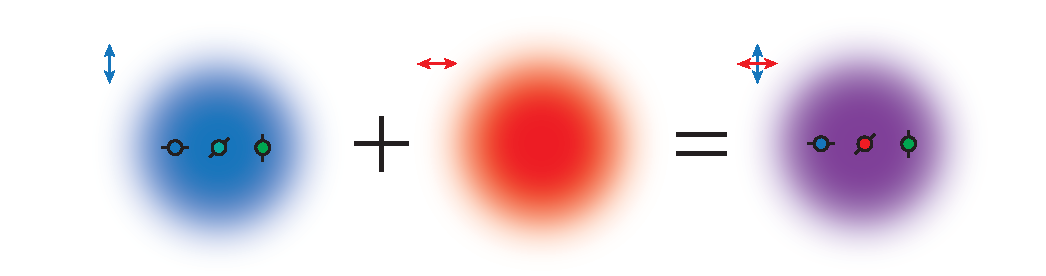
\includegraphics[width=\linewidth]{psted.pdf}
	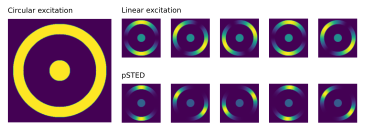
\includegraphics{psted_simulation.pdf}
	\caption{
		\textbf{Top:} Illustration of the working principle of pSTED. The arrows outside indicate the polarisation of the laser light. The circles represent fluorophores with their transition dipole moment indicated by a line. The orthogonal polarisation of the depletion beam suppresses fluorescence of the fluorophore oriented at \ang{45}.
		\textbf{Middle:} A simulation of pSTED compared to other excitation schemes on a sample consisting of a non-polarised disk and a radially polarised ring, where the excitation polarisation goes from \ang{0} to \ang{180}.
		\textbf{Bottom:} Simulation of a grid of superimposed fibres, where the fluorophores are aligned with the fibre. If the fibre spacing is below the spatial resolution, then pSTED can show the presence of two different orientations. The excitation polarisation in this figure goes from \ang{-20} to \ang{+20}.
	}
	\label{fig:psted principle}
\end{figure}

What follows is strongly inspired by Dyba et al.~\cite{Dyba2005}. Let $ \vb{x} = (x, y, z)$ be the spatial coordinates, $ \theta $ be an angle with the $ x $ axis in the $ xy $ plane (ranging from $ 0 $ to $ 2\pi$) and $ \phi $ be an angle with the $ z $ axis in the $ xz $ plane (ranging from $ -\pi$ to $+\pi$). We can also introduce a generalised coordinate $ \vb{y} = (\vb{x}, \theta, \phi) $ for a more convenient notation.
Let the fluorophore population be described by the density $ \rho(\vb{y}) $. This function is normalised such that its integral is equal to the number of fluorophores. For example, a single fluorophore at the origin, whose transition dipole points in the $ x $ direction with no out-of-plane tilt would be described by the Dirac distribution $ \rho_0 = \delta(\vb{y}) $, defined as follows:
\begin{gather}
	\delta(\vb{y}) = 0 \qq{if} y\neq0, \\
	\int f(\vb{y})\delta(\vb{y}-\vb{y}_0) \dd{\vb{y}} = f(\vb{y}_0).
\end{gather}

The excitation beam is described by the electric field amplitude $ \vb{E}_\exc $, polarised along $ \theta_\exc $, and analogous for the depletion beam. Like \autoref{eq:convolution}, the emission intensity measured when the laser is focused on $ \vb{x} $ and polarised along $ \theta $, $ \phi$ is now a convolution integral where we also have to integrate over the angles $ \theta $ and $ \phi $ like
\begin{equation}
	\begin{aligned}
		I_\emm 
			&= A \int 
				\sigma_\exc \abs{\unitvec{n}_{\theta'\phi'} \cdot \vb{E}_\exc(\vb{x}-\vb{x}')}^2 
				\rho(\vb{y}') 
				\dd{\vb{y}'} \\
			&= \int 
				\sigma_\exc I_\exc(\vb{x}'-\vb{x}) \abs{\unitvec{n}_{\theta'\phi'}\unitvec{n}_{\theta\phi}}^2
				\rho(\vb{y}') 
				\dd{\vb{y}'}
	\end{aligned}
\end{equation}
where $ \unitvec{n}_{\theta\phi} $ is a unit vector pointing in the direction of $ (\theta, \phi) $ and $ A = \epsilon_0c/2 $. $ \epsilon_0 $ is a constant denoting the vacuum permittivity. The dot product can be expressed as
\begin{equation}
	\abs{\unitvec{n}_{\theta'\phi'}\unitvec{n}_{\theta\phi}}^2 = \cos^2(\theta-\theta') \cos^2(\phi-\phi'),
\end{equation}
so we can express the emission intensity as a convolution product like
\begin{gather}
	I_\emm = (\rho*h_\exc)(\vb{y}), \\
	\qq{where} h_\exc(\vb{y}) = \sigma_\exc I_\exc(\vb{x}) \cos^2\theta\cos^2\phi.
\end{gather}
If we have a constant laser intensity $ I_\exc $ that is polarised along $ \theta_\exc $ without any out-of-plane polarisation, this reduces to
\begin{equation}
	I_\emm = \sigma_\exc I_\exc \cos^2\theta_\exc
\end{equation}
for the distribution $ \rho_0 $. $ I_\emm $ is maximal when the excitation polarisation is in the $ x $ direction, as expected. From this equation, we can derive the same angular resolution as before, but with more rigour.

Now, we need to include the effect of the polarised depletion field, which amounts to adding an exponential factor under the integral
\begin{multline}
	I_\emm = A \int
		\sigma_\exc \abs{\unitvec{n}_{\theta'\phi'} \cdot \vb{E}_\exc(\vb{x}-\vb{x}')}^2 
		\exp(-\sigma_\dep \abs{\unitvec{n}_{\theta'\phi'} \cdot \vb{E}_\dep(\vb{x}-\vb{x}')}^2)
		\rho(\vb{y}') 
		\dd{\vb{y}'}.
	\label{eq:psted integral}
\end{multline}
In essence, this is equivalent to multiplying the kernel $ h_\exc $ with the function $ \eta $
\begin{gather}
	h(\vb{y}) = h_\exc(\vb{y}) \cdot \eta(\vb{y})  \qq{, where} \\
	\eta(\vb{y}) = \exp(-\sigma_\dep I_\dep(\vb{x}) \sin^2 \theta),
\end{gather}
which assumes both electric fields are orthogonally polarised and confined to the $ xy $ plane.

\begin{figure}
	\centering
	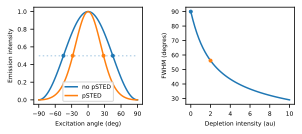
\includegraphics{pol_psf_width.pdf}
	\caption{
		\textbf{Left:} Narrowing of the fluorophore response as a result of a depletion field (of intensity $ I_\dep=2 $, as compared to the right pane). \textbf{Right:} The FWHM angular resolution $ d_\theta $ as a function of depletion intensity.
	}
	\label{fig:pol psf width}
\end{figure}

Now, we can calculate the angular resolution of this method. With a bit of algebra, it can be shown that the FWHM resolution equals
\begin{equation}
	d_\theta = 2\arccos\sqrt\frac{\mathcal{W}(k e^{k}/2)}{k},
\end{equation}
where $ k = \sigma_\dep I_\dep $ and $ \mathcal{W}(\cdot) $ denotes the Lambert W-function, the inverse of the function $ f(x) = xe^x $. As expected, $ d_\theta=\ang{90} $ for $ I_d=0 $. For other values of $ I_d $, the resolution is plotted in \autoref{fig:pol psf width}.

In an experiment, one could account for depolarising effects such as rotational diffusion, energy transfer, et cetera. That is not necessary at this point, but could be easily modelled by convolving $ \eta $ with a depolarisation kernel $ \delta $. This kernel would be a probability distribution that quantifies how much a dipole can move and rotate between absorption and interaction with the depletion beam. It is also possible to model polarisation-sensitive detection with
\begin{equation}
	h = h_\exc \cdot (\eta * \delta_1) \cdot (h_\mathit{det} * \delta_2).
\end{equation}

\section{Samples}
\label{sec:samples}

During the project, samples were very generously provided by research groups led by Pontus Nordenfelt and Vinay Swaminathan (%Division of Infection Medicine, 
Faculty of Medicine, Lund University).

Results of the cell sample shown in the experimental section contain a human cell line infected with bacteria of the Yersinia genus. Stainings present are: DAPI (tags DNA in the nucleus), GFP (tags the bacteria) and SiR-actin (tags the actin cytoskeleton). SiR-actin is an organic molecule (silicon-rhodamine) rigidly linked to an actin monomer. This dye is perfect for the setup, as SiR can be excited at 664~nm and has a sufficient absorption cross-section at 775~nm to perform STED. In addition, the fact that it is rigidly bound to the actin cytoskeleton means the light it emits is strongly polarised and reports on the actin filament orientation.

I also used two control samples for calibration measurements. The first is a sample of reflective gold colloids, which were used to image the laser point spread functions. The second contains larger Tetraspec fluorescent beads (Invitrogen).